\documentclass[11pt]{article}
\usepackage[a4paper,margin=1in]{geometry}
\usepackage{amsmath,amssymb,amsthm,mathtools}
\usepackage[expansion=false]{microtype}
\usepackage{graphicx,booktabs,array}
\usepackage[font=small,labelfont=bf]{caption}
\usepackage[dvipsnames]{xcolor}
\usepackage{enumitem}
\usepackage[hidelinks,pdfusetitle]{hyperref}
\usepackage[nameinlink,capitalise]{cleveref}
\setlist{nosep,leftmargin=1.5em}
\newtheorem{theorem}{Theorem}
\newtheorem{lemma}[theorem]{Lemma}
\newtheorem{proposition}[theorem]{Proposition}
\newtheorem{corollary}[theorem]{Corollary}
\theoremstyle{definition}\newtheorem{definition}[theorem]{Definition}
\theoremstyle{remark}\newtheorem{remark}[theorem]{Remark}
\newcommand{\R}{\mathbb R}\newcommand{\C}{\mathbb C}\newcommand{\N}{\mathbb N}
\newcommand{\dd}{\,\mathrm d}\newcommand{\e}{\mathrm e}
\newcommand{\Num}{\mathrm{Num}}\newcommand{\Den}{\mathrm{Den}}
\renewcommand{\Re}{\operatorname{Re}}\renewcommand{\Im}{\operatorname{Im}}
\setlength{\parskip}{0.35em}
\AtBeginDocument{\sloppy}
\urlstyle{same}
\hypersetup{pdftitle={The Balanced Pair in Excitable Tissue: What a Membrane Reading Determines, and the Balanced Cortex},pdfauthor={Abhijit Singh}}
\title{\textbf{The Balanced Pair in Excitable Tissue:}\\[4pt]
\large What a Membrane Reading Determines, and the Balanced Cortex}
\author{Abhijit Singh}
\date{25 September 2026}
\begin{document}
\maketitle
\begin{abstract}
Excitable tissue is read through pairs: the open and closed states of a gate, the inward and outward charges of a spike, the excitatory and inhibitory inputs of a cortical network. We prove that in a balanced network of excitatory and inhibitory neurons the residual net input and the distance of the population rates from the balance solution are one object, $\mu=\sqrt K\,A\,(\nu-\nu_{\mathrm{bal}})$, where $K$ is the number of connections per neuron and $A$ the matrix of the balance equations. In simulations of $2\times10^4$ binary neurons with $K=100$ to $1600$ this identity reproduces the measured rates to $2.67\times10^{-3}$. The excitatory and inhibitory inputs grow as $\sqrt K$ per unit rate (log--log slopes $0.4994$--$0.5004$), the net input stays of order one, and fractions $0.9763$ (E) and $0.9954$ (I) of the excitatory drive cancel at $K=1600$. The rates approach balance slowly, $40.6\%$ (E) and $22.2\%$ (I) below it at $K=1600$, exactly as the identity requires: $\det A=0.2$ amplifies the residual, and mean-field rates come within $10\%$ of balance only for $K>\text{40,054}$ (E) and $K>\text{8,897}$ (I).

The network is the top of a ladder that starts at the single gate. The two-state gate $p=1/(1+e^{-z(V-V_{1/2})})$ is balanced at its half-point, where its occupancy is $\frac12$, its entropy one bit and its variance largest. The Hodgkin--Huxley half-points are $-40.02$ ($m$), $-62.31$ ($h$) and $-53.41$ mV ($n$), and $n^4$ reaches half its maximum $34.5$ mV above the half-point of its gate. Mean currents determine only the product $Ni$ of channel number and unitary current, and the variance separates the two; the precision of the channel count improves steadily with the largest open probability reached, with no threshold at $\frac12$: it goes from no reliable estimate at $0.19$ to a factor of two at $0.5$ and $\pm12\%$ at $0.87$. Voltage-dependent block is a two-state gate whose two parameters separate affinity from electrical distance; the magnesium block of NMDA receptors has its half-point at $-20.5$ mV at $1$ mM, moving $11.2$ mV per doubling. We derive the spike threshold of exponential-onset sodium activation in closed form, $\theta=E_{\mathrm{Na}}-k_a[1-W_{-1}(-(g_L/g_{\mathrm{Na}})e^{1-(E_{\mathrm{Na}}-V_a)/k_a})]$, which reduces the error of the simplest threshold equation by a factor of $1.3$ to $33$, and show that a threshold reading fixes $V_a$ and $g_{\mathrm{Na}}$ only through $g_{\mathrm{Na}}e^{-V_a/k_a}$. The inward and outward charges of a spike cancel exactly. The sodium conductance $m^3h$ is a triad with a fourth: three activating particles, like the channel's three fast voltage sensors, and one inactivating particle, like the domain IV sensor. Its spike (amplitude $104.06$ mV) carries $13.36$ times the minimum sodium charge, and among exponents $1$ to $4$ only $m^3h$ gives both a stable rest and a spike. The sodium--potassium pump is the unequal pair $3{:}2$; it moves one elementary charge per cycle and stalls at $-205$ mV. The proofs use the two-state law, the binomial variance, the Lambert function and the balance equations; the numbers come from the Hodgkin--Huxley equations integrated to relative tolerance $10^{-9}$ and from direct simulation of the network.
\end{abstract}

\section{Introduction}\label{sec:intro}
Hodgkin and Huxley described the squid giant axon by voltage-dependent gates: three activating particles $m$ and one inactivating particle $h$ for the sodium conductance, and four particles $n$ for the potassium conductance \cite{HH}. Fluctuation analysis added a second reading of the same channels: the variance of a current carried by $N$ channels is a parabola in its mean, from which Neher and Stevens and Sigworth obtained the number of channels and their unitary current \cite{NeherStevens,Sigworth,AGL}. Woodhull described voltage-dependent block by a charged blocker that binds partway through the membrane field \cite{Woodhull}; the magnesium block of NMDA receptors \cite{Nowak,Mayer} is its best-known instance, with the empirical form of Jahr and Stevens \cite{JahrStevens}. Fourcaud-Trocm\'e et al.\ showed that spike initiation is captured by an exponential onset of sodium activation \cite{FT}, and Platkiewicz and Brette derived a threshold equation for it \cite{PB}. Fluorescence recordings placed the fast activation of the sodium channel in the voltage sensors of domains I--III and its inactivation in the sensor of domain IV \cite{ChandaBezanilla,Capes}. At the scale of the cortex, van Vreeswijk and Sompolinsky showed that a network whose excitatory and inhibitory inputs are each of order $\sqrt K$ settles into a balanced state in which they cancel to order one \cite{vVS96,vVS98}.

Each of these readings is a reading of a pair. The two-state gate has log-odds $-z(V-V_{1/2})$, which takes the values $s$ and $-s$ at $V_{1/2}\mp s/z$, with the half-point as its zero; the sum of independent gates keeps the half-point; the connectivity row $\{+1,0,-J_X\}/\sqrt K$ of the balanced network has excitatory and inhibitory members that cancel to order one; and the inactivating particle of $m^3h$ closes what the other three open. The classical questions (how many channels there are, how large a single-channel current is, where a gate activates, where a spike starts, how far a network is from balance) are therefore questions of identifiability: which parameters of the hidden pairs a reading determines, and which it confounds.

\paragraph{Companion papers.} The two-state law used here, $p=1/(1+e^{\varepsilon})$ with $\varepsilon$ the log-odds of the closed member, is the law with which \cite{Chem} reads atomic levels and gas sensors. There $\varepsilon$ is an energy difference in units of $k_BT$ (with a degeneracy term) and the half-point is a temperature. Here $\varepsilon=-z(V-V_{1/2})$ and the half-point is a voltage; for a gate moving an effective gating charge $z_g$ through the membrane field, $\varepsilon=-z_ge(V-V_{1/2})/k_BT$ is again a free-energy difference in units of $k_BT$ \cite{Hille}. The ternary rows of the cortical connectivity are weight vectors of the kind used in the ternary-weight networks of \cite{Algo}, with the magnitude split between $+1$ and $-J_X$. The synthesis paper \cite{Synth} places these results beside those of the other fields.

\subsection{Main results}\label{sec:main}
\paragraph{The balanced cortex.} In the network of van Vreeswijk and Sompolinsky (\cref{sec:net}), $N_E$ excitatory and $N_I$ inhibitory binary neurons are connected at random: a neuron of population $X\in\{E,I\}$ receives on average $K$ connections from each population, with weight $+1/\sqrt K$ from an excitatory neuron and $-J_X/\sqrt K$ from an inhibitory one, together with an external input $\sqrt K\,b_X\nu_0$. Write $\nu=(\nu_E,\nu_I)^{\!\top}$ for the population rates, $\mu=(\mu_E,\mu_I)^{\!\top}$ for the population-mean net inputs, and
\[
A=\begin{pmatrix}1&-J_E\\1&-J_I\end{pmatrix},\qquad b=\begin{pmatrix}b_E\\b_I\end{pmatrix}.
\]

\begin{theorem}[the zero and the residual]\label{thm:zero}
Let $\nu_{\mathrm{bal}}=-\nu_0A^{-1}b$, that is
\[
\nu_E^{\mathrm{bal}}=\nu_0\,\frac{J_Ib_E-J_Eb_I}{J_E-J_I},\qquad \nu_I^{\mathrm{bal}}=\nu_0\,\frac{b_E-b_I}{J_E-J_I}.
\]
(a) Both are positive if and only if $b_E/b_I>J_E/J_I>1$ or $b_E/b_I<J_E/J_I<1$.
\par\noindent(b) Up to terms of order $\sqrt K/N_E$ from the excluded self-connections, the residual net input and the rate error are one object:
\[
\mu=\sqrt K\,A\,(\nu-\nu_{\mathrm{bal}}),\qquad \nu-\nu_{\mathrm{bal}}=\frac{A^{-1}\mu}{\sqrt K}.
\]
\par\noindent(c) Hence rates that stay bounded with $\mu=O(1)$ converge to $\nu_{\mathrm{bal}}$ with error $O(1/\sqrt K)$, amplified by $A^{-1}$, whose entries scale as $1/\det A=1/(J_E-J_I)$.
\end{theorem}

We simulate the network with $N_E=N_I=10^4$, $J_E=2$, $J_I=1.8$, $b_E=1$, $b_I=0.8$ and $\nu_0=0.1$, for which $\nu_{\mathrm{bal}}=(0.1,0.1)$ and $\det A=0.2$, at $K=100$ to $1600$ (\cref{sec:net}). Inserting the measured net inputs into \cref{thm:zero}(b) reproduces the measured rates to within $2.67\times10^{-3}$ at every $K$. The excitatory and inhibitory inputs grow as $\sqrt K$ per unit rate, with log--log slopes $0.4994$--$0.5004$; their raw slopes, $1.0962$ (excitation) and $0.6774$ (inhibition) onto the E population, are $\frac12$ plus the slopes of the still-rising rates. The net input stays of order one (log--log slopes $-0.0523$ and $0.0234$), and at $K=1600$ fractions $0.9763$ (E) and $0.9954$ (I) of the excitatory drive cancel. The rates approach balance slowly, $40.6\%$ (E) and $22.2\%$ (I) below it at $K=1600$, exactly as \cref{thm:zero} requires: $A^{-1}$ multiplies the order-one residual by up to $10$, and in mean field the rates come within $10\%$ of balance only for $K>\text{40,054}$ (E) and $K>\text{8,897}$ (I). The mean net input lies $1.66$ (E) and $1.55$ (I) standard deviations of its fluctuation below threshold, so the neurons fire on fluctuations, irregularly and asynchronously.

\paragraph{The gate.} The network is the top of a ladder that starts at the single gate. A gate $x$ with opening rate $\alpha(V)$ and closing rate $\beta(V)$ relaxes to $x_\infty=\alpha/(\alpha+\beta)$ with time constant $\tau=1/(\alpha+\beta)$ \cite{HH}. Its half-point $V_{1/2}$ is where the two members exchange at equal rates, $\alpha(V_{1/2})=\beta(V_{1/2})$, and $\mathcal H(x)=-x\log_2x-(1-x)\log_2(1-x)$ is the entropy of a single gate's state.

\begin{theorem}[the gate at its half-point]\label{thm:half}
Let $\varepsilon(V)=\ln(\beta/\alpha)$ be the log-odds of the closed member.
\par\noindent(a) $x_\infty=1/(1+e^{\varepsilon})$ and $x_\infty-\frac12=-\frac12\tanh(\varepsilon/2)$.
\par\noindent(b) At $V_{1/2}$: $\varepsilon=0$, $x_\infty=\frac12$, $\tau=1/(2\alpha(V_{1/2}))$, the entropy $\mathcal H(x_\infty)$ takes its maximum, one bit, and the variance $x_\infty(1-x_\infty)$ of the gate's state takes its maximum, $\frac14$.
\par\noindent(c) $\mathrm{logit}\,x_\infty=\ln(x_\infty/(1-x_\infty))=\ln(\alpha/\beta)$. The gate has the Boltzmann form $p(V)=1/(1+e^{-z(V-V_{1/2})})$ for all $V$ if and only if $\ln(\alpha/\beta)$ is linear in $V$, and then $z=1/k$ with $k=[\frac{d}{dV}\ln(\alpha/\beta)]^{-1}$. For a general gate this $k$, evaluated at $V_{1/2}$, is the local slope factor.
\par\noindent(d) For a Boltzmann gate, $p(V_{1/2}+\Delta)+p(V_{1/2}-\Delta)=1$ for every $\Delta$, and the occupancies $\frac13$ and $\frac23$ lie at $V_{1/2}\mp k\ln2$, where the log-odds are $\pm\ln2$.
\end{theorem}

For the Hodgkin--Huxley gates the half-points are $-40.02$ ($m$), $-62.31$ ($h$) and $-53.41$ mV ($n$) (\cref{tab:hh}). A product of gates is not a pair: $n_\infty^4$ crosses $\frac12$ at $-18.88$ mV, $34.5$ mV above the half-point of $n$.

\paragraph{Channel number and unitary current.} Let $N$ independent channels each carry unitary current $i$ when open, with open probability $p$ at a fixed voltage, and let a recording add independent background noise of variance $\sigma_b^2$.

\begin{theorem}[what the mean and the variance determine]\label{thm:ident}
(a) The mean current $I=Ni\,p$ is invariant under $(N,i)\mapsto(\lambda N,i/\lambda)$ for every $\lambda>0$: no set of mean measurements determines $N$ or $i$ separately.
\par\noindent(b) The variance satisfies $\sigma^2=\sigma_b^2+iI-I^2/N$ \cite{Sigworth,NeherStevens}, and measurements at three or more distinct values of $p$ determine $(\sigma_b^2,i,N)$.
\par\noindent(c) The curvature term $I^2/N$ is a fraction $p$ of the linear term $iI$. The variance is largest, $\sigma_b^2+Ni^2/4$, at $p=\frac12$.
\end{theorem}

By (c), when $p$ stays small the parabola is nearly a line and $N$ is weakly determined. In simulated recordings of $N=2000$ channels the precision of the count improves steadily with the largest open probability $p_{\max}$ reached, and there is no threshold at the half-point: at $p_{\max}=0.19$ there is no reliable estimate, reaching $\frac12$ determines $N$ to within about a factor of two (10--90\% range $1462$--$3296$), and reaching $0.87$ to about $\pm12\%$ (\cref{tab:count}). A blocker is read in the same way: the Woodhull blocker is a Boltzmann gate whose slope and half-point separate electrical distance from affinity (\cref{prop:block}), and the magnesium block of NMDA receptors has its half-point at $-20.53$ mV at $1$ mM, moving $11.18$ mV per doubling of the concentration.

\paragraph{The threshold.} Consider $C\dot V=\Phi(V)=g_L(E_L-V)+g_\mathrm{Na}m_\infty(V)(E_\mathrm{Na}-V)$, with $m_\infty$ a Boltzmann gate of half-point $V_a$ and slope $k_a$, and let the threshold $\theta$ be the voltage where $\Phi'(\theta)=0$ \cite{PB}. Below $V_a$, $m_\infty\approx e^{(V-V_a)/k_a}$ and $1-m_\infty\approx1$; we call this the exponential approximation.

\begin{theorem}[closed-form threshold]\label{thm:thr}
In the exponential approximation:
\par\noindent(a) the threshold satisfies the fixed-point equation
\[
\theta=V_a-k_a\ln\Bigl[\frac{g_\mathrm{Na}}{g_L}\Bigl(\frac{E_\mathrm{Na}-\theta}{k_a}-1\Bigr)\Bigr],
\]
whose solution below $E_{\mathrm{Na}}-2k_a$ is
\[
\theta=E_\mathrm{Na}-k_a\Bigl[1-W_{-1}\Bigl(-\frac{g_L}{g_\mathrm{Na}}e^{1-(E_\mathrm{Na}-V_a)/k_a}\Bigr)\Bigr],
\]
with $W_{-1}$ the lower real branch of the Lambert function;
\par\noindent(b) the sodium current below $V_a$ depends on $V_a$ and $g_\mathrm{Na}$ only through $g_\mathrm{Na}e^{-V_a/k_a}$, and, given $k_a$, $E_\mathrm{Na}$ and $g_L$, the threshold and all subthreshold dynamics determine only $V_a-k_a\ln(g_\mathrm{Na}/g_L)$.
\end{theorem}

For $V_a=-30$ mV and $k_a=6$ mV the closed form reduces the error of the simplest threshold equation of \cite{PB} by a factor of $1.3$ (at $g_\mathrm{Na}/g_L=2$) to $33$ (at $14$) (\cref{tab:thr}).

\paragraph{The spike, the $3+1$ channel and the $3{:}2$ pump.} For a space-clamped membrane $C\dot V=-I_{\mathrm{Na}}-I_{\mathrm{K}}-I_{\mathrm{L}}+I_{\mathrm{stim}}$, let $Q_{\mathrm{Na}}=\int(-I_{\mathrm{Na}})\,\mathrm dt$ be the inward sodium charge and $Q_{\mathrm{K}}=\int I_{\mathrm{K}}\,\mathrm dt$, $Q_{\mathrm{L}}=\int I_{\mathrm{L}}\,\mathrm dt$, $Q_{\mathrm{stim}}=\int I_{\mathrm{stim}}\,\mathrm dt$, and let $\rho=Q_{\mathrm{Na}}/(C\,\Delta V_{\mathrm{sp}})$ compare the sodium charge of a spike of amplitude $\Delta V_{\mathrm{sp}}$ with the charge the membrane capacitance needs to reach the peak.

\begin{theorem}[the spike as a pair of charges, and the $3+1$ channel]\label{thm:charge}
(a) Over any interval whose end-points have equal voltage, $Q_{\mathrm{Na}}=Q_{\mathrm{K}}+Q_{\mathrm{L}}-Q_{\mathrm{stim}}$. Over the rising phase, from rest to the peak, $Q_{\mathrm{Na}}-Q_{\mathrm{K}}-Q_{\mathrm{L}}+Q_{\mathrm{stim}}=C\,\Delta V_{\mathrm{sp}}$.
\par\noindent(b) In the Hodgkin--Huxley model of the squid axon (\cref{sec:na}) with sodium conductance $g_{\mathrm{Na}}m^qh$ and all other parameters fixed, $q=3$ is the only exponent in $\{1,2,3,4\}$ for which the membrane has a stable resting state and fires a spike in response to a pulse of $10\ \mu$A/cm$^2$ for 1 ms. For $q=3$ the spike has amplitude $104.063$ mV and $\rho=13.3566$.
\end{theorem}

The sodium conductance $m^3h$ is thus a triad with a fourth: three identical activating particles, as the channel has three fast voltage sensors in domains I--III, and one inactivating particle, as the sensor of domain IV drives fast inactivation \cite{ChandaBezanilla,Capes}. The integrated charges of the squid spike satisfy (a) to $1.0\times10^{-16}$ of $Q_{\mathrm{Na}}$, and $87.35\%$ of the sodium charge enters after the peak.

\begin{theorem}[the pump as the unequal pair $3{:}2$]\label{thm:pump}
A pump that exports three Na$^+$ and imports two K$^+$ per cycle moves one elementary charge outwards per cycle, twice the half-difference of the pair $(3,2)$, whose common part is $\frac52$. With reversal potentials $E_\mathrm{Na}$, $E_\mathrm K$ and membrane potential $V_m$, the work against the gradients per cycle is
\[
W_{\mathrm{cyc}}=3e(E_\mathrm{Na}-V_m)+2e(V_m-E_\mathrm K)=e\,(3E_\mathrm{Na}-2E_\mathrm K-V_m),
\]
which decreases by one electron-volt per volt of $V_m$. If each cycle is driven by the free energy $|\Delta G_\mathrm{ATP}|$ of one ATP, the pump runs forward if and only if $V_m>3E_\mathrm{Na}-2E_\mathrm K-|\Delta G_\mathrm{ATP}|/e$, the stall potential, and reverses its cycle below it.
\end{theorem}

For $E_\mathrm{Na}=+55$ mV, $E_\mathrm K=-90$ mV and $V_m=-65$ mV, $W_{\mathrm{cyc}}=0.410$ eV $=15.3\,k_BT$ at $310$ K, against $0.290$ eV for a $2{:}2$ exchanger that moves no charge; with $|\Delta G_\mathrm{ATP}|\approx0.55$ eV the pump stalls at $-205$ mV, so it runs forward throughout the physiological range \cite{Nguyen,MiloPhillips}.

\subsection{Methods of proof}
\Cref{thm:half,thm:ident,thm:pump} and \cref{thm:thr}(b) are exact consequences of the two-state law: the logit of a gate, the binomial variance of $N$ gates written in terms of the mean current, the energy balance of one pump cycle, and the scaling symmetry of an exponential activation. \Cref{thm:thr}(a) reduces the threshold condition to $Ue^U=w$ and selects the branch of the Lambert function by the side of $E_{\mathrm{Na}}-2k_a$ on which the threshold lies. \Cref{thm:charge}(a) is the integral of the current equation. \Cref{thm:charge}(b) is proved by computation: the fixed points of the $m^qh$ membrane are located as roots of the steady-state current and classified by the eigenvalues of the Jacobian, and the response to the pulse is obtained by integrating the four-dimensional system at relative tolerance $10^{-9}$, reproduced by an implicit Runge--Kutta integration. \Cref{thm:zero} follows from averaging the ternary connectivity over its distribution (\cref{prop:triad}) and inverting the $2\times2$ balance matrix. The network results come from direct simulation of the binary network with asynchronous updates, and the mean-field rates from the equations of \cite{vVS98}, solved by Newton-type root finding.

\subsection{Organisation and notation}
\Cref{sec:gate} proves \cref{thm:half} and computes the Hodgkin--Huxley half-points; \cref{sec:ident} proves \cref{thm:ident} and quantifies channel counting; \cref{sec:block} treats voltage-dependent block; \cref{sec:thr} proves \cref{thm:thr}; \cref{sec:na} proves \cref{thm:charge,thm:pump}; \cref{sec:net} proves \cref{thm:zero} and reports the network; \cref{sec:interp} draws the scales together, and \cref{sec:data} lists every input. Voltages are in mV, gating rates in ms$^{-1}$, conductances in mS/cm$^2$, current densities in $\mu$A/cm$^2$ and charges in nC/cm$^2$ unless stated otherwise. $X,Y\in\{E,I\}$ label the excitatory and inhibitory populations, network inputs are in units of threshold, and time in the network is in units of the excitatory update time $\tau_E$.

\section{The gate as a pair}\label{sec:gate}
\subsection{The half-point}
Let the gate $x$, its rates $\alpha$, $\beta$, its half-point $V_{1/2}$ and the entropy $\mathcal H$ be as in \cref{sec:main}. We prove \cref{thm:half}.
\begin{proof}
(a) $x_\infty=1/(1+\beta/\alpha)=1/(1+e^{\varepsilon})$, and $x_\infty-\frac12=(1-e^{\varepsilon})/(2(1+e^{\varepsilon}))=-\frac12\tanh(\varepsilon/2)$. (b) $\alpha=\beta$ gives $\varepsilon=0$, $x_\infty=\frac12$ and $\tau=1/(2\alpha)$. $\mathcal H'(x)=\log_2((1-x)/x)$ vanishes only at $x=\frac12$ and $\mathcal H$ is strictly concave, so its maximum is $\mathcal H(\frac12)=1$. $x(1-x)=\frac14-(x-\frac12)^2\le\frac14$, with equality only at $\frac12$. (c) $x_\infty/(1-x_\infty)=\alpha/\beta$. The Boltzmann form is equivalent to $\mathrm{logit}\,p=z(V-V_{1/2})$, which is linear in $V$ with slope $z$; conversely a linear $\ln(\alpha/\beta)$ that vanishes at $V_{1/2}$ equals $(V-V_{1/2})/k$. (d) $1/(1+e^{-a})+1/(1+e^{a})=1$ for every real $a$. Next, $p=\frac13$ means $e^{-z(V-V_{1/2})}=2$, that is $V=V_{1/2}-k\ln2$, and $p=\frac23$ means $e^{-z(V-V_{1/2})}=\frac12$, that is $V=V_{1/2}+k\ln2$.
\end{proof}

\subsection{The Hodgkin--Huxley gates}
We use the rate functions of Hodgkin and Huxley \cite{HH}, shifted to a resting potential of $-65$ mV as in \cite{DayanAbbott}. With $V$ in mV and rates in $\mathrm{ms}^{-1}$,
\begin{equation}\label{eq:hh}
\begin{aligned}
\alpha_m&=\frac{0.1(V+40)}{1-e^{-(V+40)/10}}, & \beta_m&=4e^{-(V+65)/18},\\
\alpha_h&=0.07e^{-(V+65)/20}, & \beta_h&=\frac{1}{1+e^{-(V+35)/10}},\\
\alpha_n&=\frac{0.01(V+55)}{1-e^{-(V+55)/10}}, & \beta_n&=0.125e^{-(V+65)/80}.
\end{aligned}
\end{equation}
Time constants refer to the original temperature of $6.3\,^\circ$C. The half-points are the roots of $\alpha(V)=\beta(V)$, found by a bracketing root search to better than $10^{-6}$ mV. The slope $k$ follows by differentiating $\ln(\alpha/\beta)$; for example, $\frac{d}{dV}\ln\alpha_m=\frac1{V+40}-\frac{1}{10}\frac{e^{-(V+40)/10}}{1-e^{-(V+40)/10}}$ and $\frac{d}{dV}\ln\beta_m=-\frac1{18}$. The time constant at the half-point is $\tau(V_{1/2})=1/(2\alpha(V_{1/2}))$, and the $\frac13$, $\frac23$ points are the roots of $x_\infty(V)=\frac13,\frac23$ (\cref{tab:hh}).

\begin{table}[htbp]\centering\small
\caption{The Hodgkin--Huxley gates at their half-points.}\label{tab:hh}
\begin{tabular}{@{}lccccc@{}}\toprule
gate & $V_{1/2}$ (mV) & slope $k=[d\,\mathrm{logit}\,x_\infty/dV]^{-1}$ (mV) & $\tau(V_{1/2})$ (ms) & $V(\frac13)$, $V(\frac23)$ (mV) & $x_\infty(-65)$\\\midrule
$m$ & $-40.02$ & $+9.47$ & $0.50$ & $-46.43$, $-33.28$ & $0.053$\\
$h$ & $-62.31$ & $-6.95$ & $8.17$ & $-57.44$, $-67.09$ & $0.596$\\
$n$ & $-53.41$ & $+16.35$ & $4.62$ & $-63.99$, $-41.07$ & $0.318$\\\bottomrule
\end{tabular}
\end{table}

The sign of $k$ says which member opens with depolarisation ($h$ closes). The $\frac13$ and $\frac23$ points lie within $1.02$ mV of $V_{1/2}\mp k\ln2$; the largest difference is that of $n$ at $\frac23$. Further from the half-point the Hodgkin--Huxley rate functions depart from Boltzmann form. We measure the departure at occupancy $x$ as $|V(x)-V_{1/2}-k\ln(x/(1-x))|$, with $V(x)$ the root of $x_\infty(V)=x$, and evaluate it at the $161$ equally spaced occupancies from $0.1$ to $0.9$. The largest departure is $1.97$ mV for $m$, $0.84$ mV for $h$ and $14.22$ mV for $n$ (at occupancy $0.9$); for $n$ at $0.95$ it is $28.8$ mV.

\paragraph{Sums are pairs; products are not.} The mean current of $N$ independent identical gates is $Ni\,p(V)$, whose normalised form is $p(V)$ itself, with the half-point and slope of one gate (\cref{sec:ident}). A product of gates behaves differently. The steady sodium open fraction $m_\infty^3h_\infty$, evaluated on a $0.01$ mV grid from $-100$ to $40$ mV, peaks at $0.0077$ at $-31.9$ mV (the window open fraction), far below $\frac12$. The steady potassium open fraction $n_\infty^4$ crosses $\frac12$ at $-18.88$ mV, where $n_\infty=2^{-1/4}=0.841$. This is $34.5$ mV above the gate's own half-point, and the shift is the effect of taking the fourth power. An exact Boltzmann gate with the same $V_{1/2}$ and $k$ would reach $n_\infty=2^{-1/4}$ at $V_{1/2}+k\ln(2^{-1/4}/(1-2^{-1/4}))=-26.20$ mV, with $\ln(2^{-1/4}/(1-2^{-1/4}))=1.6649$; the $7.3$ mV difference is the departure of $n_\infty$ itself from Boltzmann form at $0.841$. The half-activation of a conductance measured from macroscopic current is therefore the half-point of the underlying gate only when the conductance is linear in that gate.

\begin{figure}[t]\centering
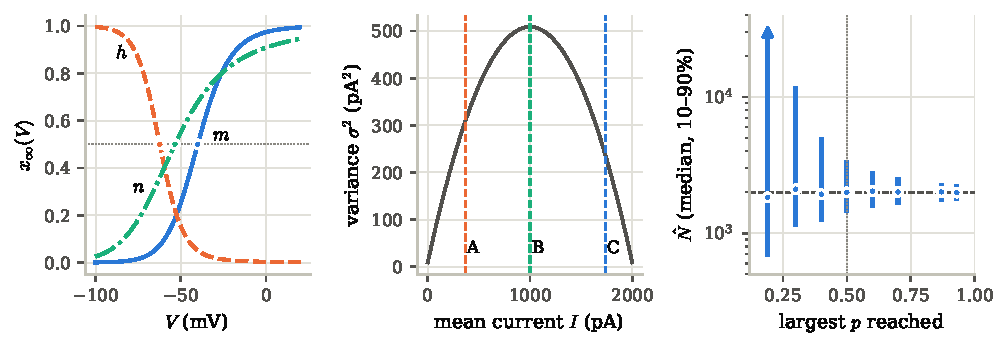
\includegraphics[width=\textwidth]{fig_membrane.pdf}
\caption{Left: steady-state Hodgkin--Huxley gates with their half-points (dots). Middle: the mean--variance parabola $\sigma^2=\sigma_b^2+iI-I^2/N$ ($N=2000$, $i=1$ pA, $\sigma_b=3$ pA); dashed lines mark the largest mean current reached when the largest open probability is $0.19$ (A), $0.50$ (B) and $0.87$ (C). Right: recovered channel number against the largest open probability reached (median and 10--90\% range over 400 simulated recordings each; failed fits are counted as $\hat N=\infty$, and the arrow marks an infinite upper quantile). Dashed: true $N$.}
\label{fig:membrane}
\end{figure}

\section{What the mean and the variance determine}\label{sec:ident}
Let $N$, $i$, $p$ and $\sigma_b^2$ be as in \cref{thm:ident}. Because the unitary current depends on the driving force, the theorem is stated at a fixed voltage, where $p$ is varied in time (as in nonstationary fluctuation analysis, for example during a voltage step). Across voltages the same statements hold in conductance units, $\sigma_G^2=\sigma_b^2/(V-E_\mathrm{rev})^2+\gamma G-G^2/N$, with $\gamma$ the unitary conductance and $G$ the mean conductance; this is again linear in $(\sigma_b^2,\gamma,1/N)$.

We prove \cref{thm:ident}.
\begin{proof}
(a) $(\lambda N)(i/\lambda)p=Nip$. (b) The number of open channels is binomial with mean $Np$ and variance $Np(1-p)$, so the current has variance $\sigma_b^2+i^2Np(1-p)$. Substituting $p=I/(Ni)$ gives $i^2N\frac{I}{Ni}(1-\frac{I}{Ni})=iI-I^2/N$. The right side is a polynomial of degree two in $I$ with coefficients $(\sigma_b^2,i,-1/N)$. Distinct values of $p$ give distinct values of $I$, and a polynomial of degree at most two is fixed by its values at three distinct points (the $3\times3$ Vandermonde matrix is invertible). (c) $(I^2/N)/(iI)=I/(Ni)=p$. Also $\frac{d}{dI}(iI-I^2/N)=0$ at $I=Ni/2$, that is at $p=\frac12$, where the variance is $\sigma_b^2+Ni^2/4$.
\end{proof}

By \cref{thm:ident}(c), when $p$ stays small the parabola is nearly a line and $N$ is weakly determined. To quantify this we simulated recordings of $N=2000$ channels with $i=1$ pA and $\sigma_b=3$ pA. Their open probability follows the Boltzmann gate $p(V)=1/(1+e^{-(V+40)/9.47})$, which has the half-point and slope of the $m$ gate, rounded. A recording consists of 9 voltages spaced linearly from $-80$ mV to $V_{\max}=-40+9.47\ln(p_{\max}/(1-p_{\max}))$ mV, the voltage at which $p$ reaches its largest value $p_{\max}$, with 200 independent sweeps at each voltage. In each sweep the number of open channels is drawn from the binomial distribution with parameters $N$ and $p(V)$. The current is $i$ times that number plus an independent normal deviate of mean $0$ and standard deviation $\sigma_b$. At each voltage we form the sample mean $I$ and the unbiased sample variance $\sigma^2$ of the 200 currents. We then fit $\sigma^2=\eta_0+\eta_1I-\eta_2I^2$ to the 9 pairs $(I,\sigma^2)$ by ordinary (unweighted) least squares, giving $\hat\imath=\eta_1$ and $\hat N=1/\eta_2$. A fit fails when $\eta_2\le0$, and such fits are counted as $\hat N=\infty$. For each $p_{\max}$ we generated 400 independent recordings and report the 10\%, 50\% and 90\% quantiles of $\hat N$ (\cref{tab:count}).

\begin{table}[htbp]\centering\small
\caption{Recovered channel number against the largest open probability reached ($N=2000$; 400 simulated recordings per design).}\label{tab:count}
\begin{tabular}{@{}lcccccccc@{}}\toprule
$p_{\max}$ & $0.19$ & $0.30$ & $0.40$ & $0.50$ & $0.60$ & $0.70$ & $0.87$ & $0.93$\\\midrule
$\hat N$, 10\% & $699$ & $1160$ & $1270$ & $1462$ & $1613$ & $1687$ & $1770$ & $1809$\\
$\hat N$, median & $1834$ & $2105$ & $1935$ & $1996$ & $2039$ & $2010$ & $2009$ & $1988$\\
$\hat N$, 90\% & $\infty$ & $11592$ & $4904$ & $3296$ & $2748$ & $2472$ & $2240$ & $2193$\\
failed fits & $20.5\%$ & $6.5\%$ & $1.5\%$ & $0$ & $0$ & $0$ & $0$ & $0$\\\bottomrule
\end{tabular}
\end{table}

These quantiles are themselves Monte Carlo estimates from 400 recordings. In ten independent repetitions of the whole experiment every quantile for $p_{\max}\ge0.5$ stayed within $10\%$ of the tabulated value, and the failure fraction stayed at or below $0.5\%$. For $p_{\max}\le0.4$ the 90\% quantile lies in a heavy tail and varied by up to $20\%$ ($p_{\max}=0.4$) and several-fold ($0.3$); at $p_{\max}=0.19$ the median varied by up to $25\%$ and the failure fraction between $18\%$ and $27\%$. None of the conclusions below depends on these variations. The unitary current is recovered in each of the three designs of \cref{fig:membrane} (voltages from $-80$ mV to $-54$, $-40$ and $-22$ mV, that is $p_{\max}=0.19$, $0.50$, $0.87$; 400 recordings each; median $\hat\imath$ between $0.985$ and $1.001$ pA), because it is the slope of the parabola at the origin. The precision of $\hat N$ improves steadily with $p_{\max}$, and there is no threshold at the half-point. Reaching $p=\frac12$ determines $N$ to within about a factor of two (10--90\% range $1462$--$3296$); reaching $0.87$ determines it to about $\pm12\%$; at $0.19$ there is no reliable estimate. A precise channel count needs open probabilities well above $\frac12$ \cite{AGL}.

\section{Voltage-dependent block}\label{sec:block}
Consider a blocker of valence $z_{\mathrm{bl}}$ applied from the outside. It binds without permeating at electrical distance $\delta$ from the outside, with zero-voltage dissociation constant $K_{\mathrm d}(0)$ ($V$ is the inside potential relative to the outside). The site feels the fraction $\delta$ of the membrane potential, so the dissociation constant is $K_{\mathrm d}(V)=K_{\mathrm d}(0)e^{z_{\mathrm{bl}}\delta FV/RT}$, and the fraction of channels left unblocked is \cite{Woodhull}
\[
B(V)=\frac1{1+[\mathrm B]/K_{\mathrm d}(V)}=\frac1{1+([\mathrm B]/K_{\mathrm d}(0))\,e^{-z_{\mathrm{bl}}\delta FV/RT}}.
\]

\begin{proposition}[the blocker as a gate]\label{prop:block}
$B(V)$ is a Boltzmann gate, $B(V)=1/(1+e^{-(V-V_{1/2})/k_{\mathrm{bl}}})$, with slope $k_{\mathrm{bl}}=RT/(z_{\mathrm{bl}}\delta F)$ and half-point $V_{1/2}=k_{\mathrm{bl}}\ln([\mathrm B]/K_{\mathrm d}(0))$. A change of affinity $K_{\mathrm d}(0)\mapsto\kappa K_{\mathrm d}(0)$ moves the half-point by $-k_{\mathrm{bl}}\ln\kappa$ at fixed slope. A change of electrical distance $\delta\mapsto c\,\delta$ divides both $k_{\mathrm{bl}}$ and $V_{1/2}$ by $c$. Doubling the blocker concentration moves the half-point by $k_{\mathrm{bl}}\ln2$.
\end{proposition}
\begin{proof}
With $k_{\mathrm{bl}}=RT/(z_{\mathrm{bl}}\delta F)$, $([\mathrm B]/K_{\mathrm d}(0))e^{-V/k_{\mathrm{bl}}}=e^{-(V-V_{1/2})/k_{\mathrm{bl}}}$ exactly when $V_{1/2}=k_{\mathrm{bl}}\ln([\mathrm B]/K_{\mathrm d}(0))$. The three statements follow from this formula: $\ln([\mathrm B]/(\kappa K_{\mathrm d}(0)))=\ln([\mathrm B]/K_{\mathrm d}(0))-\ln\kappa$; $k_{\mathrm{bl}}$ is proportional to $1/\delta$; and $\ln(2[\mathrm B])=\ln[\mathrm B]+\ln2$.
\end{proof}

For the magnesium block of NMDA receptors \cite{Nowak,Mayer}, the standard empirical form $B(V)=1/(1+[\mathrm{Mg^{2+}}]/3.57\,\mathrm{mM}\cdot e^{-0.062V/\mathrm{mV}})$ \cite{JahrStevens} gives $k_{\mathrm{bl}}=1/0.062=16.13$ mV and $K_{\mathrm d}(0)=3.57$ mM, and $V_{1/2}=k_{\mathrm{bl}}\ln([\mathrm{Mg^{2+}}]/3.57\,\mathrm{mM})$ (\cref{tab:mg}).

\begin{table}[htbp]\centering\small
\caption{Magnesium block of NMDA receptors as a two-state gate.}\label{tab:mg}
\begin{tabular}{@{}lccc@{}}\toprule
$[\mathrm{Mg^{2+}}]$ (mM) & $V_{1/2}$ (mV) & $B(-70\ \mathrm{mV})$ & $B(-20\ \mathrm{mV})$\\\midrule
$0.5$ & $-31.71$ & $0.085$ & $0.674$\\
$1.0$ & $-20.53$ & $0.044$ & $0.508$\\
$2.0$ & $-9.35$ & $0.023$ & $0.341$\\\bottomrule
\end{tabular}
\end{table}

Each doubling moves the half-point by $k_{\mathrm{bl}}\ln2=11.18$ mV. At room temperature ($295$ K), $RT/F=25.42$ mV (with $R$ and $F$ from \cite{CODATA}), so the slope corresponds to $z_{\mathrm{bl}}\delta=(RT/F)/k_{\mathrm{bl}}=1.58$, that is $\delta\approx0.8$ for the divalent ion. At a resting potential of $-65$ mV the receptor is held almost entirely in its blocked member, $44.5$ mV below the half-point at $1$ mM. This is why its current requires the coincidence of glutamate binding and postsynaptic depolarisation. The two-state form describes an impermeant blocker. Magnesium also permeates the channel at strongly negative voltages \cite{AntonovJohnson}, which adds a second exit from the blocked state and relieves the block there.

\section{The spike threshold}\label{sec:thr}
Let $\Phi$, $m_\infty$, $V_a$, $k_a$ and the threshold $\theta$, the voltage where $\Phi'(\theta)=0$, be as in \cref{thm:thr}, following Platkiewicz and Brette \cite{PB} (see also \cite{FT}). Since $m_\infty'=m_\infty(1-m_\infty)/k_a$,
\[
\Phi'(V)=-g_L+g_\mathrm{Na}m_\infty(V)\Bigl[\frac{(E_\mathrm{Na}-V)(1-m_\infty(V))}{k_a}-1\Bigr].
\]
Below $V_a$, $m_\infty\approx e^{(V-V_a)/k_a}$ and $1-m_\infty\approx1$. In this exponential approximation $\Phi'(\theta)=0$ becomes $g_\mathrm{Na}e^{(\theta-V_a)/k_a}[(E_\mathrm{Na}-\theta)/k_a-1]=g_L$.

We prove \cref{thm:thr}(a).
\begin{proof}
Taking logarithms of $g_\mathrm{Na}e^{(\theta-V_a)/k_a}[(E_\mathrm{Na}-\theta)/k_a-1]=g_L$ gives the fixed-point equation. Substitute $y=(E_\mathrm{Na}-\theta)/k_a-1$, so that $\theta=E_\mathrm{Na}-k_a(1+y)$ and $(\theta-V_a)/k_a=(E_\mathrm{Na}-V_a)/k_a-1-y$. The equation $e^{(\theta-V_a)/k_a}y=g_L/g_\mathrm{Na}$ becomes $ye^{-y}=(g_L/g_\mathrm{Na})e^{1-(E_\mathrm{Na}-V_a)/k_a}$, that is $(-y)e^{-y}=w$ with $w=-(g_L/g_\mathrm{Na})e^{1-(E_\mathrm{Na}-V_a)/k_a}$. For $w\in(-1/e,0)$ the equation $Ue^U=w$ has exactly two real solutions, $U=W_0(w)\in(-1,0)$ and $U=W_{-1}(w)<-1$ \cite{Corless}. Hence $y=-W_0(w)\in(0,1)$ or $y=-W_{-1}(w)>1$. The first gives $\theta>E_\mathrm{Na}-2k_a$. The second gives $\theta<E_\mathrm{Na}-2k_a$ and the stated formula.
\end{proof}

For the parameters below, $w$ lies between $-10^{-6}$ and $-10^{-7}$. The branch $W_0$ gives $\theta=49.0$ mV, far above $V_a$, where the exponential approximation does not hold; the branch $W_{-1}$ gives the threshold. Fixed points and bifurcations of exponential integrate-and-fire models are analysed in \cite{TouboulBrette}. With an exponential nonlinearity such fixed-point conditions are of Lambert type, and the form here carries the sodium driving force. Replacing $E_\mathrm{Na}-\theta$ by $E_\mathrm{Na}-V_a$ and dropping the $-1$ gives the simplest form of the threshold equation of \cite{PB}, $\theta\approx V_a-k_a\ln[(g_\mathrm{Na}/g_L)(E_\mathrm{Na}-V_a)/k_a]$.

We take $V_a=-30$ mV and $k_a=6$ mV, within the ranges quoted in \cite{PB} ($V_a$ about $-30$ mV, $k_a=4$--$8$ mV for neuronal sodium channels), and the illustrative values $E_\mathrm{Na}=55$ mV and $E_L=-70$ mV. The exact $\theta$ is the root of the full $\Phi'(V)=0$ below $V_a$ (with the Boltzmann $m_\infty$), found by a bracketing root search on $[-150,V_a]$ mV. For $V<\theta$, $\Phi'<0$, so $\Phi$ decreases from $+\infty$ to its minimum $\Phi(\theta)$, and a resting state ($\Phi=0$ below $\theta$) exists if and only if $\Phi(\theta)<0$. Solving $\Phi(\theta)=0$ as a function of $g_\mathrm{Na}/g_L$ shows that the model has a resting state exactly for $g_\mathrm{Na}/g_L<14.65$; above that, $\Phi$ has no zero below $\theta$ and $\theta$ is the minimum of $\Phi$. \Cref{tab:thr} covers the range with a resting state (errors are approximation minus exact).

\begin{table}[htbp]\centering\small
\caption{Spike threshold: exact root, simplest threshold equation and closed form.}\label{tab:thr}
\begin{tabular}{@{}lccccccc@{}}\toprule
$g_\mathrm{Na}/g_L$ & 2 & 4 & 6 & 8 & 10 & 12 & 14\\\midrule
exact $\theta$ (mV) & $-50.63$ & $-55.27$ & $-57.92$ & $-59.78$ & $-61.21$ & $-62.38$ & $-63.37$\\
simplest form, error (mV) & $+0.56$ & $+1.04$ & $+1.26$ & $+1.39$ & $+1.49$ & $+1.57$ & $+1.63$\\
closed form, error (mV) & $-0.42$ & $-0.19$ & $-0.12$ & $-0.09$ & $-0.07$ & $-0.06$ & $-0.05$\\\bottomrule
\end{tabular}
\end{table}

The closed form reduces the error of the simplest form by a factor of $1.3$ (at $g_\mathrm{Na}/g_L=2$) to $33$ (at $14$). Its remaining error is that of the exponential approximation to $m_\infty$, and it shrinks as $\theta$ moves below $V_a$.

We prove \cref{thm:thr}(b), which states what a threshold reading determines.
\begin{proof}
$g_\mathrm{Na}e^{(V-V_a)/k_a}=(g_\mathrm{Na}e^{-V_a/k_a})e^{V/k_a}$, which is unchanged when $V_a$ moves by $\Delta$ and $g_\mathrm{Na}$ is multiplied by $e^{\Delta/k_a}$. In part (a) the argument of $W_{-1}$ is $-e^{1-E_\mathrm{Na}/k_a}\,e^{(V_a-k_a\ln(g_\mathrm{Na}/g_L))/k_a}$.
\end{proof}

\section{The spike as a pair: the \texorpdfstring{$3+1$}{3+1} sodium channel and the \texorpdfstring{$3{:}2$}{3:2} pump}\label{sec:na}
\paragraph{Background.} Hodgkin and Huxley described the sodium conductance as $g_{\mathrm{Na}}m^3h$: three identical activation particles and one inactivation particle \cite{HH}. The voltage-gated sodium channel is one polypeptide with four homologous domains, I--IV, each with a voltage sensor \cite{Hille}; its primary voltage sensor comprises four positively charged S4 segments \cite{ChandaBezanilla}. Fluorescence near the S4 segments of domains I, II and III has a fast component comparable to the fast gating current, and the three signals start together. The domain IV signal follows the slow gating component with a lag, a later step in the activation sequence \cite{ChandaBezanilla}. Movement of the domain IV sensor is the rate-limiting step for the development of and recovery from fast inactivation, and its activation alone is sufficient for fast inactivation \cite{Capes}. The overlap of inward and outward currents is the largest component of the energetic cost of the squid-axon spike in Hodgkin--Huxley-type models \cite{Crotty}, and sodium entry relative to its capacitive minimum is a standard measure of spike efficiency \cite{Alle}.

We prove \cref{thm:charge}(a).
\begin{proof}
Integrate the current equation: $\int C\dot V\,\mathrm dt=C\,\Delta V$, which is $0$ in the first case and $C\,\Delta V_{\mathrm{sp}}$ in the second.
\end{proof}
$C\,\Delta V_{\mathrm{sp}}$ is the charge the membrane capacitance needs to reach the peak. The ratio $\rho=Q_{\mathrm{Na}}/(C\,\Delta V_{\mathrm{sp}})$ compares the sodium charge with it, and $Q_{\mathrm{Na}}-C\,\Delta V_{\mathrm{sp}}$ is the sodium charge cancelled by outward current.

\paragraph{The squid-axon spike.} The membrane is
\[
C\dot V=-g_{\mathrm{Na}}m^3h(V-E_{\mathrm{Na}})-g_{\mathrm{K}}n^4(V-E_{\mathrm{K}})-g_{\mathrm{L}}(V-E_{\mathrm{L}})+I_{\mathrm{stim}},
\]
with $\dot x=\alpha_x(V)(1-x)-\beta_x(V)x$ for $x=m,h,n$ and the rate functions \eqref{eq:hh}. The standard squid parameters are $C=1\ \mu$F/cm$^2$, $g_{\mathrm{Na}}=120$, $g_{\mathrm{K}}=36$, $g_{\mathrm{L}}=0.3$ mS/cm$^2$, $E_{\mathrm{Na}}=50$, $E_{\mathrm{K}}=-77$ and $E_{\mathrm{L}}=-54.387$ mV \cite{HH,DayanAbbott}. The equations, together with the cumulative integrals of the three ionic currents and of $I_{\mathrm{stim}}$, are integrated numerically by an adaptive stiff/non-stiff multistep method (relative tolerance $10^{-9}$, absolute $10^{-11}$, step at most $0.01$ ms), and the solution is read on a $1\ \mu$s grid. An independent integration by an implicit Runge--Kutta (Radau) method reproduces the $m^3h$ values below to the digits quoted. The resting state is the fixed point of the four-dimensional system at $I_{\mathrm{stim}}=0$, found as the root of the steady-state current and confirmed stable by the eigenvalues of the Jacobian: the membrane rests at $-64.996$ mV. The stimulus starts at $t=1$ ms. The amplitude is $\Delta V_{\mathrm{sp}}=V_{\mathrm{peak}}-V_{\mathrm{rest}}$, and the width is the full width at $V_{\mathrm{rest}}+\Delta V_{\mathrm{sp}}/2$. Charges are integrated from stimulus onset to the first return of $V$ to $V_{\mathrm{rest}}$ after the peak. The 1-ms threshold is the smallest pulse amplitude for which $V$ exceeds $0$ mV within 10 ms of onset, found by bisection.

A pulse of $10\ \mu$A/cm$^2$ for 1 ms (threshold $6.919\ \mu$A/cm$^2$) gives a spike peaking at $39.067$ mV: amplitude $104.063$ mV, width at half amplitude $1.4544$ ms (\cref{fig:cortex}c). From onset to repolarisation the membrane takes in $Q_{\mathrm{Na}}=1389.934$ nC/cm$^2$ of sodium charge against $C\,\Delta V_{\mathrm{sp}}=104.063$ nC/cm$^2$: $\rho=13.3566$ ($13.4663$ over a 20 ms window). The rising phase alone uses $1.6901\,C\,\Delta V_{\mathrm{sp}}$, and $87.35\%$ of the sodium charge enters after the peak. At the peak of the inward sodium current ($787.6\ \mu$A/cm$^2$, at $2.911$ mV) the potassium current is $821.2\ \mu$A/cm$^2$, and the net ionic current is $0.0645$ of the sodium current. \Cref{thm:charge}(a), evaluated with the integrated charges, holds to $1.0\times10^{-16}$ of $Q_{\mathrm{Na}}$, that is to rounding error.

\paragraph{The number of activating particles.} We replace $m^3$ by $m^q$ in the sodium current, with all other parameters fixed (\cref{tab:exp}, \cref{fig:cortex}d). Fixed points are the roots of the steady-state current on $[-100,50]$ mV, bracketed on a $0.005$-mV grid and refined by Brent's method, with stability from the eigenvalues of the Jacobian. For $q=2$ the limit cycle is obtained by integrating for 400 ms from 1 mV above the fixed point. Its period is averaged over the cycles in the last 200 ms, and $\rho$ per cycle is the sodium charge per cycle divided by $C$ times the peak-to-trough amplitude.

\begin{table}[htbp]\centering\small
\caption{The sodium conductance $m^qh$ for $q=1,\dots,4$, other parameters fixed.}\label{tab:exp}
\begin{tabular}{@{}clllll@{}}\toprule
$q$ & fixed point (mV) & standard stimulus & amplitude (mV) & width (ms) & $\rho$\\\midrule
1 & $-40.32$, stable & no spike & -- & -- & --\\
2 & $-47.43$, unstable & periodic firing & $115.346^a$ & $1.60$ & $14.0119^a$\\
3 & $-65.00$, stable & spike & $104.063$ & $1.4544$ & $13.3566$\\
4 & $-65.83$, stable & no spike & $104.533^b$ & $1.4635^b$ & $11.9407^b$\\\bottomrule
\end{tabular}\\[2pt]
{\footnotesize $^a$Peak to trough and per cycle of the limit cycle. $^b$At $1.5$ times the $m^4h$ 1-ms threshold of $22.326\ \mu$A/cm$^2$, that is at $33.489\ \mu$A/cm$^2$.}
\end{table}

With one activating particle the steady window current holds the membrane at $-40.32$ mV with the inactivation gate almost closed ($h=0.0522$). The standard pulse moves it by $1.072$ mV, and it crosses $0$ mV only when driven by a pulse $70.99$ times the $m^3h$ threshold: there is no regenerative spike. With two particles no resting state is stable, and the membrane fires spontaneously with period $10.4268$ ms. With four the rest is stable, and the standard pulse gives only $7.363$ mV because the threshold is $3.227$ times higher; above threshold the spike is almost unchanged. Among the spiking cases $\rho$ is $14.0119$ ($q=2$, per cycle), $13.3566$ ($q=3$) and $11.9407$ ($q=4$). Within the fitted model of \cite{HH}, whose other parameters were fitted with three activating particles, $q=3$ is the only exponent that gives both a stable rest and a spike to the standard stimulus. This proves \cref{thm:charge}(b).

\paragraph{The pump as the unequal pair \texorpdfstring{$3{:}2$}{3:2}.} The sodium--potassium pump exports three Na$^+$ and imports two K$^+$ per ATP hydrolysed \cite{Nguyen}. We prove \cref{thm:pump}.
\begin{proof}
As a pair $(3,2)$ the stoichiometry has common part $\frac52$ and half-difference $\pm\frac12$, and the net charge moved outwards per cycle, $3-2=1$ elementary charge, is twice the half-difference. Moving one Na$^+$ from inside to outside against its electrochemical gradient costs $e(E_\mathrm{Na}-V_m)$, and moving one K$^+$ from outside to inside costs $e(V_m-E_\mathrm K)$. Summing over the three and the two ions gives $W_{\mathrm{cyc}}=e(3E_\mathrm{Na}-2E_\mathrm K-V_m)$, whose derivative in $V_m$ is $-e$: one electron-volt per volt, because one net charge is moved outwards. The cycle runs forward when the free energy supplied exceeds the work against the gradients, $|\Delta G_\mathrm{ATP}|>W_{\mathrm{cyc}}$, that is when $V_m>3E_\mathrm{Na}-2E_\mathrm K-|\Delta G_\mathrm{ATP}|/e$; at equality it stalls, and below it the net cycle reverses.
\end{proof}
With the illustrative values $E_\mathrm{Na}=+55$ mV, $E_\mathrm K=-90$ mV and $V_m=-65$ mV, and potentials in volts so that the costs are in eV, the work against the gradients per cycle is
\[
W_{\mathrm{cyc}}=3(E_\mathrm{Na}-V_m)+2(V_m-E_\mathrm K)=0.360+0.050=0.410\ \text{eV}=15.3\,k_BT\ \text{at }310\ \text{K}.
\]
A $2{:}2$ exchanger would do $2\cdot0.120+2\cdot0.025=0.290$ eV and move no charge. With $|\Delta G_\mathrm{ATP}|\approx0.55$ eV per ATP ($53$ kJ\,mol$^{-1}$, within the range of about $47$--$70$ kJ\,mol$^{-1}$ for cells collected in \cite{MiloPhillips}), the pump stalls where $W_{\mathrm{cyc}}=|\Delta G_\mathrm{ATP}|$, at $V_m=3E_\mathrm{Na}-2E_\mathrm K-0.55\,\mathrm V=-205$ mV, and reverses its cycle at more negative potentials. It therefore operates forward throughout the physiological range. Exporting the sodium that enters during one squid-axon spike takes $Q_{\mathrm{Na}}/(3e)=2.89\times10^{12}$ pump cycles, and as many ATP molecules, per cm$^2$ of membrane.

\begin{figure}[t]\centering
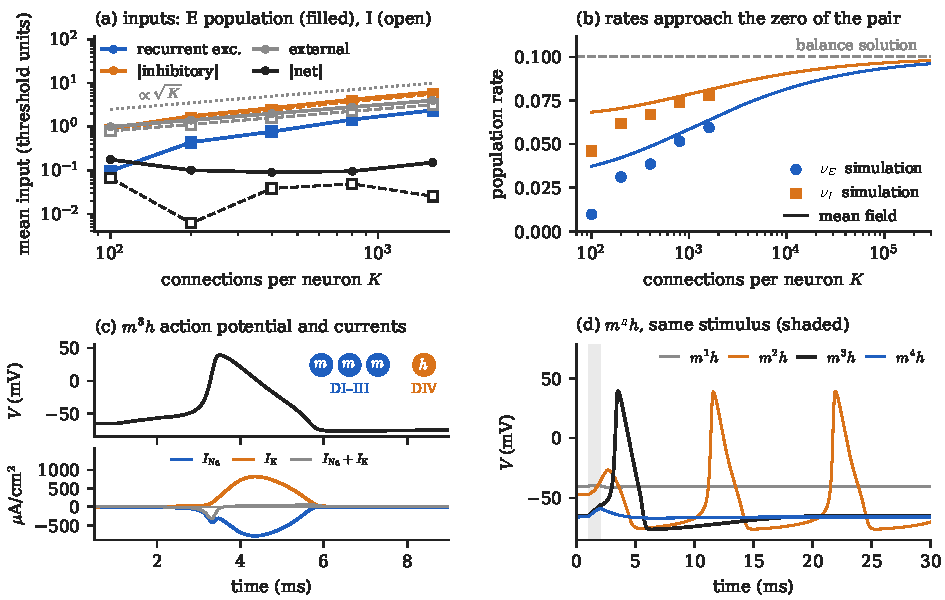
\includegraphics[width=\textwidth]{fig_cortex.pdf}
\caption{(a) Mean inputs against $K$; E population filled, I open (recurrent excitation is the same for both); the dotted line has slope $\frac12$ ($\propto\sqrt K$). External input grows as $\sqrt K$ by construction; excitation and inhibition grow faster here because the rates are still rising; the net input stays of order one. (b) Population rates $\nu_E$, $\nu_I$ and the balance solution $0.1$; lines: mean-field theory. (c) The $m^3h$ action potential (Hodgkin--Huxley squid parameters, $6.3\,^\circ$C) with its sodium and potassium currents and their sum; inset: three activating particles (domains I--III), one inactivating (domain IV). (d) $m^qh$, $q=1,\dots,4$, other parameters fixed, same $10\ \mu$A/cm$^2$, 1 ms stimulus.}\label{fig:cortex}
\end{figure}

\section{The balanced cortex as the zero of a pair}\label{sec:net}
\paragraph{Background.} Van Vreeswijk and Sompolinsky \cite{vVS96,vVS98} studied networks of $N_E$ excitatory and $N_I$ inhibitory binary neurons. Each neuron receives on average $K\ll N_E,N_I$ connections of strength $O(1/\sqrt K)$ from each population, and an external excitatory input of order $\sqrt K$. The excitatory and inhibitory inputs are then each of order $\sqrt K$, far above threshold, yet a balance between them emerges dynamically for a wide range of parameters. The large inhibitory input nearly cancels the large excitatory one, the net input is of order threshold, and the network is in an asynchronous chaotic state with irregular, fluctuation-driven firing. To leading order the rates solve linear balance equations.

\paragraph{Model.} Neuron $j$ of population $X\in\{E,I\}$ has state $S_j\in\{0,1\}$ and input
\[
u_j=\frac1{\sqrt K}\Bigl(\sum_{l\in E}c_{jl}\,S_l-J_X\sum_{l\in I}c_{jl}\,S_l\Bigr)+\sqrt K\,b_X\nu_0,
\qquad S_j\leftarrow\Theta(u_j-\theta_X),
\]
with $\Theta$ the unit step, $c_{jl}=1$ independently with probability $K/N_Y$ for $l$ in population $Y$ (and $0$ otherwise), $J_E=2$, $J_I=1.8$, $b_E=1$, $b_I=0.8$, $\nu_0=0.1$, $\theta_E=1$ and $\theta_I=0.7$. The population rates $\nu_E$, $\nu_I$ are the fractions of active neurons, and $\nu$, $\mu$, $A$ and $b$ are as in \cref{sec:main}.

\begin{proposition}[the triad of weights]\label{prop:triad}
Every row of the connectivity matrix takes values in $\{+1,0,-J_X\}/\sqrt K$. Averaged over the connectivity, the mean excitatory and inhibitory inputs to population $X$ are $\sqrt K\,\nu_E$ and $-\sqrt K\,J_X\nu_I$, up to $O(\sqrt K/N_E)$ terms from the excluded self-connections. The population-mean net input is therefore $\mu=\sqrt K\,(b\,\nu_0+A\,\nu)+O(\sqrt K/N_E)$.
\end{proposition}
\begin{proof}
An entry of row $j$ is $0$ when $c_{jl}=0$, $+1/\sqrt K$ for an excitatory $l$ with $c_{jl}=1$, and $-J_X/\sqrt K$ for an inhibitory one. Each presynaptic neuron adds $K/N_Y$ in expectation to each postsynaptic count, so summing over population $Y$ gives $K$ times its rate, less $KS_j/N_Y$ for a self-connection. Dividing by $\sqrt K$ and adding the external input gives $\mu$.
\end{proof}

We prove \cref{thm:zero}.
\begin{proof}
The balance solution is defined by $b\,\nu_0+A\,\nu_{\mathrm{bal}}=0$, that is $\nu_E-J_E\nu_I=-b_E\nu_0$ and $\nu_E-J_I\nu_I=-b_I\nu_0$. Subtracting the second equation from the first gives $(J_E-J_I)\nu_I=(b_E-b_I)\nu_0$, and then $\nu_E=J_E\nu_I-b_E\nu_0=\nu_0(J_Ib_E-J_Eb_I)/(J_E-J_I)$. Here $\det A=J_E-J_I$ and
\[
A^{-1}=\frac1{J_E-J_I}\begin{pmatrix}-J_I&J_E\\-1&1\end{pmatrix}.
\]
(a) All parameters are positive. If $J_E>J_I$, positivity needs $b_E>b_I$ and $J_Ib_E>J_Eb_I$, and the second implies the first; the case $J_E<J_I$ reverses both inequalities. (b) $b\,\nu_0=-A\,\nu_{\mathrm{bal}}$; insert this in \cref{prop:triad}. (c) is (b) read with $\mu=O(1)$.
\end{proof}
Our parameters give $b_E/b_I=1.2500>J_E/J_I=1.1111>1$, $\nu_E^{\mathrm{bal}}=\nu_I^{\mathrm{bal}}=0.1$, $\det A=0.2$ and
\[
A^{-1}=\begin{pmatrix}-9&10\\-5&5\end{pmatrix}.
\]
Each row is a ternary weight vector in the sense of \cite{Algo}. Its expected fraction of zero entries is $1-K/N_Y$ in each population block, from $0.99$ at $K=100$ to $0.84$ at $K=1600$ for the networks below.

\paragraph{Simulation method.} $N_E=N_I=10^4$ and $K\in\{100,200,400,800,1600\}$, so $K/N_E$ ranges from $0.01$ to $0.16$ (the largest network has 63,992,591 synapses). Each connection $c_{jl}$, $l\ne j$, is drawn once, independently, with probability $K/N_Y$, and each neuron starts active with probability $\nu_0$. Each E (I) neuron updates at Poisson times of rate $1/\tau_E$ ($1/\tau_I$), with $\tau_E=1$ (about $10$ ms) and $\tau_I=0.9$. This is approximated by steps $\mathrm dt=0.01\,\tau_E$ in which each neuron updates independently with probability $\mathrm dt/\tau_X$, using the inputs at the start of the step. The synaptic counts $\sum_{l\in E}c_{jl}S_l$ and $\sum_{l\in I}c_{jl}S_l$ are integers; they are updated at every change of state and agree exactly with a full recount at the end of each simulation. We discard $10\,\tau_E$ and measure over $40\,\tau_E$, sampling every $0.1\,\tau_E$ (400 samples). Connectivity, initial state and update times come from one fixed pseudo-random sequence for each $K$. The population rate $\nu_X$ is the fraction of active neurons in population $X$, averaged over the samples. An input component is its value averaged over the neurons of a population and over the samples. A log--log slope is the least-squares slope of $\log|\cdot|$ against $\log K$ over the five values of $K$. With $\mathrm dt=0.002$ the rates at $K=1600$ are $0.05922$ and $0.07774$ (against $0.05944$ and $0.07782$).

\paragraph{(a) The components and the zero.} At $K=1600$ (\cref{tab:net}, \cref{fig:cortex}a) the E population receives $2.3768$ (recurrent excitation) $+\,4.0000$ (external) $-\,6.2254$ (inhibition) $=0.1514$, and the I population $2.3770+3.2000-5.6024=-0.0254$. The net input is thus a fraction $0.0237$ (E) and $0.0046$ (I) of the excitatory drive: fractions $0.9763$ and $0.9954$ of it cancel. The net input has log--log slopes $-0.0523$ (E) and $0.0234$ (I), so it stays of order one. The excitatory and inhibitory inputs grow as $\sqrt K$ per unit rate: the per-unit-rate components $\text{exc}/\nu_E$ and $|\text{inh}|/(J_X\nu_I)$ have log--log slopes $0.4999$ and $0.5003$ (E) and $0.5004$ and $0.4994$ (I), and divided by $\sqrt K$ they lie between $0.9986$ and $1.0020$ at every $K$. The raw slopes of the components, $1.0962$ and $1.0966$ (excitation) and $0.6774$ and $0.6765$ (inhibition), reflect the still-rising rates: $\nu_E$ grows with slope $0.5963$ and $\nu_I$ with $0.1771$, and by \cref{prop:triad} a component's slope is $\frac12$ plus the slope of its rate.

\begin{table}[htbp]\centering\small\setlength{\tabcolsep}{4.5pt}
\caption{Mean inputs (threshold units) and rates; relative error $(\nu-\nu_{\mathrm{bal}})/\nu_{\mathrm{bal}}$. Mean field (MF, large $N_E$, $N_I$ \cite{vVS98}): $\nu_X=H((\theta_X-\mu_X)/\sqrt{\Sigma_X})$, with $\mu$ from \cref{prop:triad}, $\Sigma_X=\nu_E+J_X^2\nu_I$ and $H(x)=\frac12\operatorname{erfc}(x/\sqrt2)$ the Gaussian tail. The two equations are solved for $(\nu_E,\nu_I)$ by Newton-type root finding started at $\nu_{\mathrm{bal}}$, to a residual below $10^{-13}$.}\label{tab:net}
\begin{tabular}{@{}rrrrrrrrr@{}}\toprule
$K$ & exc. & inh.\ (E) & net (E) & net (I) & $\nu_E$ (rel.\ err.) & $\nu_I$ (rel.\ err.) & MF $\nu_E$ & MF $\nu_I$\\\midrule
100 & $0.0969$ & $-0.9202$ & $0.1767$ & $0.0660$ & $0.00970$ ($-0.9030$) & $0.04606$ ($-0.5394$) & $0.03731$ & $0.06834$\\
200 & $0.4408$ & $-1.7544$ & $0.1006$ & $-0.0062$ & $0.03115$ ($-0.6885$) & $0.06200$ ($-0.3800$) & $0.04224$ & $0.07050$\\
400 & $0.7714$ & $-2.6811$ & $0.0903$ & $-0.0385$ & $0.03858$ ($-0.6142$) & $0.06701$ ($-0.3299$) & $0.04866$ & $0.07361$\\
800 & $1.4613$ & $-4.1943$ & $0.0954$ & $-0.0489$ & $0.05169$ ($-0.4831$) & $0.07411$ ($-0.2589$) & $0.05615$ & $0.07737$\\
1600 & $2.3768$ & $-6.2254$ & $0.1514$ & $-0.0254$ & $0.05944$ ($-0.4056$) & $0.07782$ ($-0.2218$) & $0.06398$ & $0.08137$\\\bottomrule
\end{tabular}
\end{table}

\paragraph{(b) Rates and the balance solution.} The rates approach $\nu_{\mathrm{bal}}=0.1$ monotonically and slowly (\cref{tab:net}, \cref{fig:cortex}b): at $K=1600$ they are $40.6\%$ (E) and $22.2\%$ (I) below it, exactly as \cref{thm:zero}(b) requires. Inserting the measured population-mean net inputs $\mu$ into $\nu=\nu_{\mathrm{bal}}+A^{-1}\mu/\sqrt K$ reproduces the measured rates to within $2.67\times10^{-3}$ at every $K$ ($1.45\times10^{-4}$ at $K=1600$); the remainder is the quenched spread of out-degrees. The residual is of order one, and $A^{-1}$ multiplies it by up to $10$. At $K=1600$ the simulated rates lie $7.10\%$ (E) and $4.35\%$ (I) below the mean-field values. In one further simulation with $N_E=N_I=2\times10^4$ ($K/N_E=0.08$) they move towards them, to $0.06110$ and $0.07927$, so this gap is a finite-$K/N_E$ effect. In mean field the rate error falls below $10\%$ only for $K>\text{40,054}$ (E) and $K>\text{8,897}$ (I), the roots in $K$ of $|\nu_X-0.1|=0.01$. As $K\to\infty$, $\nu_X\to0.1$, so the mean-field equation forces $(\theta_X-\mu_X)/\sqrt{\Sigma_X}\to H^{-1}(0.1)=1.28155$ with $\Sigma_X=0.1(1+J_X^2)$, that is $\mu_E\to0.0938$ and $\mu_I\to-0.1345$. By \cref{thm:zero}(b), $\sqrt K$ times the relative error then tends to $A^{-1}\mu_\infty/0.1=(-21.891,\,-11.415)$ for (E, I). Over our range the slopes of $\log|\nu-\nu_{\mathrm{bal}}|$, $-0.2821$ (E) and $-0.3118$ (I), are pre-asymptotic.

\paragraph{(c) Irregularity: firing driven by the residual.} At $K=1600$ the net input fluctuates in time with standard deviation $0.5108$ (E) and $0.4691$ (I) (the standard deviation of each neuron's net input over the 400 samples, averaged over the population). Its mean lies $1.6613$ (E) and $1.5462$ (I) standard deviations below threshold, so the neurons fire only on fluctuations: the fraction of time the net input exceeds threshold is $0.06032$ (E) and $0.07784$ (I), close to the rates $0.05944$ and $0.07782$. Time-averaged single-neuron activities are broadly spread: mean $0.0594$, standard deviation $0.0702$ (coefficient of variation $1.182$) in E and $0.0778$, $0.0800$ (coefficient of variation $1.028$) in I, with $32.21\%$ of E and $22.53\%$ of I neurons below $0.01$. The single-neuron autocorrelation decays with $1/e$ time $1.171\,\tau_E$ (E) and $1.104\,\tau_E$ (I), close to the update time. It is computed from the activity fluctuations of 1000 recorded neurons per population, averaged over neurons, at lags that are multiples of $0.1\,\tau_E$, and the $1/e$ time is found by linear interpolation. The population activity fluctuates over the samples with standard deviation $0.00290$ (E) and $0.00164$ (I), against $\sqrt{\nu_X(1-\nu_X)/N_X}=0.00236$ and $0.00268$ for independent neurons. The two are of the same order: the state is asynchronous.

\section{Discussion: the pair, the triad and the fourth across the scales}\label{sec:interp}
\emph{The pair and its zero.} At the gate, the two members are balanced at the half-point, where the log-odds is zero, the occupancy $\frac12$, the entropy one bit and the fluctuation largest (\cref{thm:half}). A membrane reading determines a gate's half-point and slope from its mean. It determines the unitary current from fluctuations at any open probability, and the number of channels increasingly well the further the gate is driven beyond its half-point (\cref{sec:ident}). It separates a blocker's affinity from its electrical distance through the two parameters of one Boltzmann pair (\cref{prop:block}). It determines the spike threshold only through $g_\mathrm{Na}e^{-V_a/k_a}$ (\cref{thm:thr}(b)). In the network, excitation and inhibition are $s$ and $-s$. Each is of order $\sqrt K$, exactly $\sqrt K$ per unit rate, and their sum with the external drive is of order one. The balance solution is the rate vector at which the zero is exact at order $\sqrt K$.

\emph{The merge.} Adding independent identical gates keeps the pair: the normalised mean current is $p(V)$ with the half-point of one gate, and the variance of the sum is largest at the same half-point (\cref{thm:ident}). Multiplying gates does not keep it ($n_\infty^4$, \cref{sec:gate}).

\emph{The triad.} Each connectivity row is ternary, $\{+1,0,-J_X\}/\sqrt K$ (\cref{prop:triad}), and the zero of the network is built from these triads. The same three-valued alphabet carries the ternary-weight networks and balanced-ternary arithmetic of \cite{Algo}.

\emph{The residual.} What is not cancelled drives the output. Neurons fire when the order-one net input fluctuates above threshold, and \cref{thm:zero} shows that the same residual sets the distance from the zero, $\nu-\nu_{\mathrm{bal}}=A^{-1}\mu/\sqrt K$. In our range of $K$ the inputs are balanced while the rates are still approaching the balance solution; $\det A=J_E-J_I$ sets how far $K$ must grow. At the spike, the inward sodium charge equals the outward potassium and leak charge less the stimulus charge, exactly, over any interval that returns to the starting voltage (\cref{thm:charge}(a)). The voltage excursion is the part of the sodium charge not yet cancelled, and the cost of the spike, $\rho=13.36$, is the overlap of the two members. The pump restores the gradients as the unequal pair $3{:}2$, whose half-difference is the one net charge it moves per cycle.

\emph{The fourth element.} In $m^3h$ three identical members open the channel and a fourth closes it. In the channel, three sensors move together and fast, and the fourth moves later and is, on its own, sufficient and rate limiting for fast inactivation \cite{ChandaBezanilla,Capes}: it closes what the other three open. In the network, each neuron reads a zero-sum ternary input, and its output becomes an entry of other neurons' ternary rows: the observer of one triad is a member of the next.

\paragraph{Outlook.} \Cref{thm:zero} turns a recording of excitatory and inhibitory currents into a reading of how far a circuit sits from its balance solution, and the next step is to apply it to spiking networks with conductance-based synapses and to recorded cortical currents. For channel counting, recordings that drive the gate well beyond its half-point give the largest gain in precision.

\section{Data and sources}\label{sec:data}
No experimental data set is used. Every number is computed from the following inputs by the formulas and procedures stated in the text.
\begin{itemize}
\item \emph{Hodgkin--Huxley rate functions}: the fits of Hodgkin and Huxley for the squid giant axon at $6.3\,^\circ$C \cite{HH}, in the form shifted to a resting potential of $-65$ mV given in \cite[Ch.~5]{DayanAbbott}, as written in \eqref{eq:hh}; used in \cref{sec:gate,sec:na}.
\item \emph{Hodgkin--Huxley membrane parameters} \cite{HH,DayanAbbott}: $C=1\ \mu$F/cm$^2$; $g_{\mathrm{Na}}=120$, $g_{\mathrm{K}}=36$, $g_{\mathrm{L}}=0.3$ mS/cm$^2$; $E_{\mathrm{Na}}=50$, $E_{\mathrm{K}}=-77$, $E_{\mathrm{L}}=-54.387$ mV. The stimulus ($10\ \mu$A/cm$^2$ for 1 ms) is a chosen value.
\item \emph{Magnesium block}: the empirical form $B(V)=1/(1+[\mathrm{Mg^{2+}}]/3.57\,\mathrm{mM}\cdot e^{-0.062V/\mathrm{mV}})$ of Jahr and Stevens \cite{JahrStevens}, that is $K_{\mathrm d}(0)=3.57$ mM and $k_{\mathrm{bl}}=1/0.062$ mV; the concentrations $0.5$, $1$ and $2$ mM and the temperature $295$ K used for $RT/F$ are chosen values.
\item \emph{Physical constants} (CODATA 2018 \cite{CODATA}, all exact in the SI): $k_B=8.617333262\times10^{-5}$ eV\,K$^{-1}$, $R=8.314462618$ J\,mol$^{-1}$\,K$^{-1}$, $F=96485.33212$ C\,mol$^{-1}$, $e=1.602176634\times10^{-19}$ C.
\item \emph{Threshold model}: $V_a=-30$ mV and $k_a=6$ mV, within the ranges quoted in \cite{PB}; $E_\mathrm{Na}=55$ mV and $E_L=-70$ mV are illustrative values; the ratios $g_\mathrm{Na}/g_L$ are chosen.
\item \emph{Sodium--potassium pump}: stoichiometry $3$ Na$^+$ out, $2$ K$^+$ in per ATP \cite{Nguyen}; $E_\mathrm{Na}=+55$ mV, $E_\mathrm K=-90$ mV, $V_m=-65$ mV and the temperature $310$ K are illustrative values; $|\Delta G_\mathrm{ATP}|\approx0.55$ eV per molecule, within the cellular range collected in \cite{MiloPhillips}.
\item \emph{Simulated recordings} (\cref{sec:ident}): model values $N=2000$, $i=1$ pA, $\sigma_b=3$ pA, gate $V_{1/2}=-40$ mV and $k=9.47$ mV (the $m$ gate of \cref{tab:hh}, rounded), 9 voltages per recording, 200 sweeps per voltage and 400 recordings per design, all chosen. The recordings are pseudo-random samples generated as described in the text and contain no external input.
\item \emph{Network parameters} (\cref{sec:net}): the binary-network model of \cite{vVS96,vVS98}. Its parameter values ($N_E=N_I=10^4$, $K=100$--$1600$, $J_E=2$, $J_I=1.8$, $b_E=1$, $b_I=0.8$, $\nu_0=0.1$, $\theta_E=1$, $\theta_I=0.7$, $\tau_E=1$, $\tau_I=0.9$, $\mathrm dt=0.01\,\tau_E$) are chosen values. $H^{-1}(0.1)=1.28155$ is the upper $10\%$ point of the standard normal distribution.
\end{itemize}


\begin{thebibliography}{99}\small
\bibitem{HH} A.~L.~Hodgkin, A.~F.~Huxley, A quantitative description of membrane current and its application to conduction and excitation in nerve, \emph{J. Physiol.} 117(4) (1952) 500--544. doi:10.1113/jphysiol.1952.sp004764
\bibitem{NeherStevens} E.~Neher, C.~F.~Stevens, Conductance fluctuations and ionic pores in membranes, \emph{Annu. Rev. Biophys. Bioeng.} 6 (1977) 345--381. doi:10.1146/annurev.bb.06.060177.002021
\bibitem{Sigworth} F.~J.~Sigworth, The variance of sodium current fluctuations at the node of Ranvier, \emph{J. Physiol.} 307 (1980) 97--129. doi:10.1113/jphysiol.1980.sp013426
\bibitem{AGL} O.~Alvarez, C.~Gonz\'alez, R.~Latorre, Counting channels: a tutorial guide on ion channel fluctuation analysis, \emph{Adv. Physiol. Educ.} 26(4) (2002) 327--341. doi:10.1152/advan.00006.2002
\bibitem{Woodhull} A.~M.~Woodhull, Ionic blockage of sodium channels in nerve, \emph{J. Gen. Physiol.} 61 (1973) 687--708. doi:10.1085/jgp.61.6.687
\bibitem{Nowak} L.~Nowak, P.~Bregestovski, P.~Ascher, A.~Herbet, A.~Prochiantz, Magnesium gates glutamate-activated channels in mouse central neurones, \emph{Nature} 307 (1984) 462--465. doi:10.1038/307462a0
\bibitem{Mayer} M.~L.~Mayer, G.~L.~Westbrook, P.~B.~Guthrie, Voltage-dependent block by Mg$^{2+}$ of NMDA responses in spinal cord neurones, \emph{Nature} 309 (1984) 261--263. doi:10.1038/309261a0
\bibitem{JahrStevens} C.~E.~Jahr, C.~F.~Stevens, Voltage dependence of NMDA-activated macroscopic conductances predicted by single-channel kinetics, \emph{J. Neurosci.} 10 (1990) 3178--3182. doi:10.1523/JNEUROSCI.10-09-03178.1990
\bibitem{FT} N.~Fourcaud-Trocm\'e, D.~Hansel, C.~van Vreeswijk, N.~Brunel, How spike generation mechanisms determine the neuronal response to fluctuating inputs, \emph{J. Neurosci.} 23 (2003) 11628--11640. doi:10.1523/JNEUROSCI.23-37-11628.2003
\bibitem{PB} J.~Platkiewicz, R.~Brette, A threshold equation for action potential initiation, \emph{PLoS Comput. Biol.} 6(7) (2010) e1000850. doi:10.1371/journal.pcbi.1000850
\bibitem{ChandaBezanilla} B.~Chanda, F.~Bezanilla, Tracking voltage-dependent conformational changes in skeletal muscle sodium channel during activation, \emph{J. Gen. Physiol.} 120(5) (2002) 629--645. doi:10.1085/jgp.20028679
\bibitem{Capes} D.~L.~Capes, M.~P.~Goldschen-Ohm, M.~Arcisio-Miranda, F.~Bezanilla, B.~Chanda, Domain IV voltage-sensor movement is both sufficient and rate limiting for fast inactivation in sodium channels, \emph{J. Gen. Physiol.} 142(2) (2013) 101--112. doi:10.1085/jgp.201310998
\bibitem{vVS96} C.~van Vreeswijk, H.~Sompolinsky, Chaos in neuronal networks with balanced excitatory and inhibitory activity, \emph{Science} 274 (1996) 1724--1726. doi:10.1126/science.274.5293.1724
\bibitem{vVS98} C.~van Vreeswijk, H.~Sompolinsky, Chaotic balanced state in a model of cortical circuits, \emph{Neural Comput.} 10(6) (1998) 1321--1371. doi:10.1162/089976698300017214
\bibitem{Synth} A.~Singh, What a Zero Is: One Involution across Mathematics, Physics, Chemistry, Neuroscience, Computation and the Giant Planets, manuscript, 25 September 2026.
\bibitem{Chem} A.~Singh, Which Member Carries: Two-State Pairs from Atoms to Gas Sensors, and D\"obereiner's Triads as Balanced Pairs, manuscript, 25 September 2026.
\bibitem{Hille} B.~Hille, \emph{Ion Channels of Excitable Membranes}, 3rd ed., Sinauer, Sunderland MA, 2001.
\bibitem{Algo} A.~Singh, Three Is Enough: Radix Economy, Balanced-Ternary Arithmetic and Ternary-Weight Networks, manuscript, 25 September 2026.
\bibitem{Nguyen} P.~T.~Nguyen, C.~Deisl, M.~Fine et al., Structural basis for gating mechanism of the human sodium-potassium pump, \emph{Nat. Commun.} 13 (2022) 5293. doi:10.1038/s41467-022-32990-x
\bibitem{MiloPhillips} R.~Milo, R.~Phillips, \emph{Cell Biology by the Numbers}, Garland Science, New York, 2016; section ``How much energy is released in ATP hydrolysis?'', \url{https://book.bionumbers.org/how-much-energy-is-released-in-atp-hydrolysis/} (accessed 24 September 2026).
\bibitem{DayanAbbott} P.~Dayan, L.~F.~Abbott, \emph{Theoretical Neuroscience: Computational and Mathematical Modeling of Neural Systems}, MIT Press, Cambridge MA, 2001.
\bibitem{CODATA} E.~Tiesinga, P.~J.~Mohr, D.~B.~Newell, B.~N.~Taylor, CODATA recommended values of the fundamental physical constants: 2018, \emph{Rev. Mod. Phys.} 93 (2021) 025010. doi:10.1103/RevModPhys.93.025010
\bibitem{AntonovJohnson} S.~M.~Antonov, J.~W.~Johnson, Permeant ion regulation of \emph{N}-methyl-D-aspartate receptor channel block by Mg$^{2+}$, \emph{Proc. Natl. Acad. Sci. USA} 96(25) (1999) 14571--14576. doi:10.1073/pnas.96.25.14571
\bibitem{Corless} R.~M.~Corless, G.~H.~Gonnet, D.~E.~G.~Hare, D.~J.~Jeffrey, D.~E.~Knuth, On the Lambert $W$ function, \emph{Adv. Comput. Math.} 5 (1996) 329--359. doi:10.1007/BF02124750
\bibitem{TouboulBrette} J.~Touboul, R.~Brette, Dynamics and bifurcations of the adaptive exponential integrate-and-fire model, \emph{Biol. Cybern.} 99 (2008) 319--334. doi:10.1007/s00422-008-0267-4
\bibitem{Crotty} P.~Crotty, T.~Sangrey, W.~B.~Levy, Metabolic energy cost of action potential velocity, \emph{J. Neurophysiol.} 96(3) (2006) 1237--1246. doi:10.1152/jn.01204.2005
\bibitem{Alle} H.~Alle, A.~Roth, J.~R.~P.~Geiger, Energy-efficient action potentials in hippocampal mossy fibers, \emph{Science} 325 (2009) 1405--1408. doi:10.1126/science.1174331
\end{thebibliography}
\end{document}
